\section{Casi d'uso}
\subsection{Scopo}
L'obbiettivo di questa sezione è quello di presentare e descrivere tutti i casi d'uso, individuati dal team, in riferimento alle funzionalità richieste nell'applicazione.
\subsection{Attori}
Non essendo richiesto nessun tipo di servizio di autenticazione o più in generale una distinzione gerarchica degli utenti, è presente un solo attore nella gerarchia ovvero: l'utente generico.
\begin{figure}[h!]
    \centering
    
\includegraphics[scale=0.50]{../../assets/Utente.png}
    \caption{Gerarchia attori}
\end{figure}

% --------------------------------------------------------------------
% INIZIO CASI D'USO
% CARICAMENTO DATASET
% --------------------------------------------------------------------

\subsection{UC1 - Caricamento dataset}
\begin{figure}[h!]
    \centering
    % Sistema immagine inserendo tag UC e abbelliscila dc
    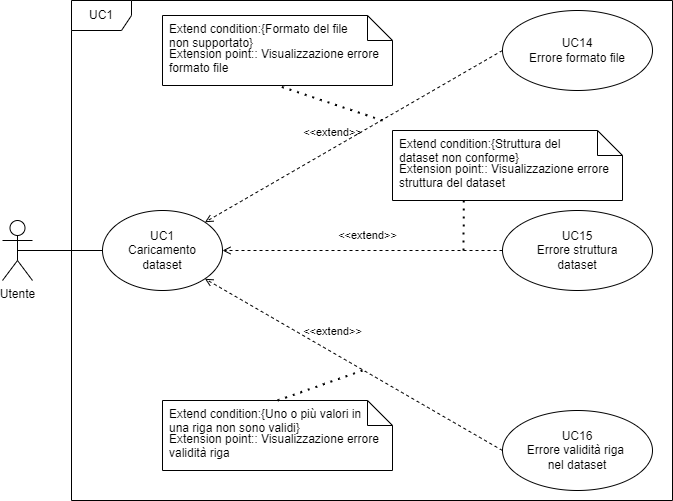
\includegraphics[scale=0.55]{../../assets/Caricamento_dataset.png}
    \caption{UC1 - Caricamento dataset}
\end{figure}
\begin{itemize}
    \item \textbf{Attore primario:} Utente.
    \item \textbf{Precondizioni:} Il sistema è funzionante
    \item \textbf{Postcondizioni:} Viene visualizzato un messaggio che avvisa l'utente del corretto caricamento dei dati e della loro validità. 
                                   I dati vengono caricati nel sistema
    \item \textbf{Scenario principale:}
          \begin{enumerate}
              \item L'utente seleziona il file da caricare
              \item L'utente carica il file
          \end{enumerate}
    \item \textbf{Estensioni:}
    \begin{itemize}
        \item   Nel caso in cui l'utente carichi un file in un formato non supportato
                \begin{enumerate}
                    \item I dati non vengono caricati
                    \item Viene visualizzato un messaggio di errore esplicativo [\hyperref[sec:UC - Errore formato file]{UC}] % To Do: metti il link alla sezione   
                \end{enumerate}
        \item   Nel caso in cui l'utente carichi un file non correttamente strutturato
                \begin{enumerate}
                    \item I dati non vengono caricati
                    \item Viene visualizzato un messaggio di errore esplicativo [\hyperref[sec:UC - Errore struttura dataset]{UC}]
                \end{enumerate}
        \item   Nel caso in cui i dati di una o più righe non siano validi
                \begin{enumerate}
                    \item Viene visualizzato un messaggio di errore esplicativo % [\hyperref[sec:UC - Errore validità riga]{UC}]  To Do: metti il link alla sezione
                \end{enumerate}
    \end{itemize} 
\end{itemize}
\newpage

% --------------------------------------------------------------------
% SCELTA TIPO GRAFICO
% --------------------------------------------------------------------

\subsection{UC2 - Scelta tipologia grafico}
\label{sec:UC2}
\begin{figure}[h!]
    \centering
    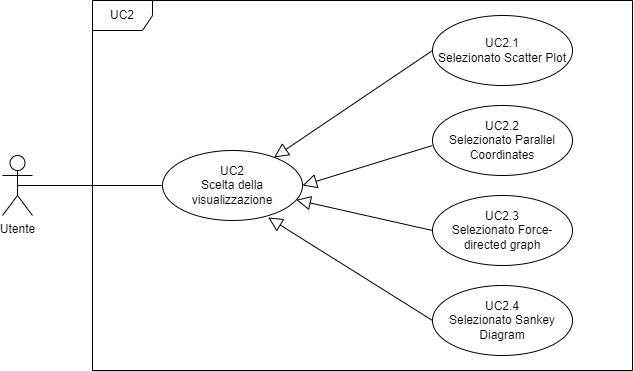
\includegraphics[scale=0.55]{../../assets/Selezione_tipo_grafico.png}
    \caption{UC2 - Scelta tipologia grafico}
\end{figure}
\begin{itemize}
    \item \textbf{Attore primario}: Utente.
    \item \textbf{Precondizioni}: Il dataset è stato caricato correttamente.
    \item \textbf{Postcondizioni}: Viene mostrata la visualizzazione scelta.
    \item \textbf{Scenario principale}:
          \begin{enumerate}
              \item L'utente seleziona il tipo di grafico da visualizzare tra le tipologie disponibili.
          \end{enumerate}
    \item \textbf{Generalizzazioni}:
    \begin{itemize}
        \item L'utente seleziona una delle seguenti opzioni:
                \begin{enumerate}
                    \item \textit{Scatter Plot} \hyperref[sec:UC2.1]{UC2.1}.
                    \item \textit{Parallel Coordinates} \hyperref[sec:UC2.2]{UC2.2}.
                    \item \textit{Force-directed Graph} \hyperref[sec:UC2.3]{UC2.3}.
                    \item \textit{Sankey Diagram} \hyperref[sec:UC2.4]{UC2.4}.
                \end{enumerate}
    \end{itemize} 
\end{itemize}

\subsubsection{UC2.1 - Selezionato Scatter Plot}
\label{sec:UC2.1}
\begin{itemize}
    \item \textbf{Attore primario}: Utente.
    \item \textbf{Precondizioni}: Il dataset è stato caricato correttamente [UC2].
    \item \textbf{Postcondizioni}: Viene mostrata la visualizzazione \textit{Scatter Plot} scelta dall'utente con possibilità di selezionare una diversa vista \hyperref[sec:UC6]{UC6} e personalizzare lo stile \hyperref[sec:UC5.1]{UC5.1}. %inserire il numero corretto dello stile e delle dimensioni
    \item \textbf{Scenario principale}:
          \begin{enumerate}
              \item L'utente seleziona il grafico \textit{Scatter Plot} e il sistema ritorna tale grafico con conseguente possibilità di personalizzazione. 
          \end{enumerate}
\end{itemize}

\subsubsection{UC2.2 - Selezionato Parallel Coordinates}
\label{sec:UC2.2}
\begin{itemize}
    \item \textbf{Attore primario}: Utente.
    \item \textbf{Precondizioni}: Il dataset è stato caricato correttamente [UC2].
    \item \textbf{Postcondizioni}: Viene mostrata la visualizzazione \textit{Parallel Coordinates} scelta dall'utente con possibilità di selezionare una diversa vista \hyperref[sec:UC6]{UC6} e personalizzare lo stile \hyperref[sec:UC5.2]{UC5.2}. %inserire il numero corretto dello stile e delle dimensioni
    \item \textbf{Scenario principale}:
          \begin{enumerate}
              \item L'utente seleziona il grafico \textit{Parallel Coordinates} e il sistema ritorna tale grafico con conseguente possibilità di personalizzazione. 
          \end{enumerate}
\end{itemize}

\subsubsection{UC2.3 - Selezionato Force-directed Graph}
\label{sec:UC2.3}
\begin{itemize}
    \item \textbf{Attore primario}: Utente.
    \item \textbf{Precondizioni}: Il dataset è stato caricato correttamente [UC2].
    \item \textbf{Postcondizioni}: Viene mostrata la visualizzazione \textit{Force-directed Graph} scelta dall'utente con possibilità di selezionare una diversa vista \hyperref[sec:UC6]{UC6} e personalizzare lo stile \hyperref[sec:UC5.3]{UC5.3}. %inserire il numero corretto dello stile e delle dimensioni
    \item \textbf{Scenario principale}:
          \begin{enumerate}
              \item L'utente seleziona il grafico \textit{Force-directed Graph} e il sistema ritorna tale grafico con conseguente possibilità di personalizzazione. 
          \end{enumerate}
\end{itemize}

\subsubsection{UC2.4 - Selezionato Sankey Diagram}
\label{sec:UC2.4}
\begin{itemize}
    \item \textbf{Attore primario}: Utente.
    \item \textbf{Precondizioni}: Il dataset è stato caricato correttamente [UC2].
    \item \textbf{Postcondizioni}: Viene mostrata la visualizzazione \textit{Sankey Diagram} scelta dall'utente con possibilità di selezionare una diversa vista \hyperref[sec:UC6]{UC6} e personalizzare lo stile \hyperref[sec:UC5.4]{UC5.4}. %inserire il numero corretto dello stile e delle dimensioni
    \item \textbf{Scenario principale}:
          \begin{enumerate}
              \item L'utente seleziona il grafico \textit{Sankey Diagram} e il sistema ritorna tale grafico con conseguente possibilità di personalizzazione. 
          \end{enumerate}
\end{itemize}
\newpage

%               _ _              _       _                 _
%  ___  ___ ___| | |_ __ _    __| | __ _| |_ __ _ ___  ___| |_
% / __|/ __/ _ \ | __/ _` |  / _` |/ _` | __/ _` / __|/ _ \ __|
% \__ \ (_|  __/ | || (_| | | (_| | (_| | || (_| \__ \  __/ |_
% |___/\___\___|_|\__\__,_|  \__,_|\__,_|\__\__,_|___/\___|\__|


\subsection{UC3 - Selezione Vista}
\label{sec:UC6}
\begin{figure}[h!]
    \centering
    % Controlla che UC abbia il numero corretto
    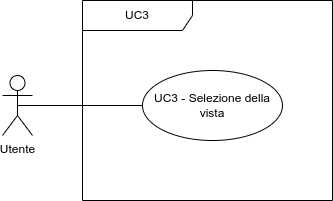
\includegraphics[scale=0.55]{../../assets/scelta_vista.png}
    \caption{UC3 - Scelta della vista dei dati da visualizzare}
\end{figure}
\begin{itemize}
    \item \textbf{Attore primario}: Utente.
    \item \textbf{Precondizioni}: Il dataset è stato caricato correttamente.
    \item \textbf{Postcondizioni}: Viene mostrata all'utente la vista dei dati selezionata.
    \item \textbf{Scenario principale}:
          \begin{enumerate}
              \item L'utente apre il menù a tendina contenente tutte le interpretazioni disponibili.
              \item L'utente seleziona la vista che vuole visualizzare.
          \end{enumerate}
\end{itemize}
\newpage

% --------------------------------------------------------------------
% VISUALIZZAZIONE DI DEFAULT DEI GRAFICI
% --------------------------------------------------------------------

\subsection{UC4 - Visualizzazione di default dei grafici}
\begin{figure}[h!]
    \centering
    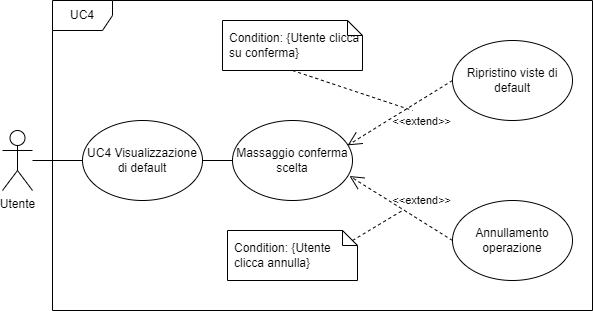
\includegraphics[scale=0.55]{../../assets/visualizzazione_default.png}
	\caption{UC4 - Visualizzazione di default dei grafici}
\end{figure}

\begin{itemize}
	\item \textbf{Attore primario:} Utente.
	\item \textbf{Precondizioni:} Il dataset è presente e caricato correttamente.
	\item \textbf{Postcondizioni:} 
	Vengono riportati i grafici alla visualizzazione di default.
	\item \textbf{Scenario principale:}
	\begin{itemize}
		\item   L'utente sceglie di ripristinare le viste
	\begin{enumerate}
		\item L'utente clicca sul pulsante di ripristino
		\item Viene visualizzato un messaggio di riconferma
		\item L'utente clicca "OK" per confermare la scelta
		\item I grafici vengono resettati alla vista di default
	\end{enumerate}
		\item   L'utente sceglie di annullare l'operazione
	\begin{enumerate}
		\item L'utente clicca sul pulsante di ripristino
		\item Viene visualizzato un messaggio di riconferma
		\item L'utente clicca "ANNULLA" per annullare l'operazione
		\item Ritorno alla vista corrente senza modifiche apportate
	\end{enumerate}	
	\end{itemize}
\end{itemize}

\newpage

% --------------------------------------------------------------------
% SEZIONE PERSONALIZZAZIONE VISIVA DEI GRAFICI
% --------------------------------------------------------------------

\subsection{UC5 - Personalizzazione visiva dei grafici}
\begin{figure}[h!]
	\centering
	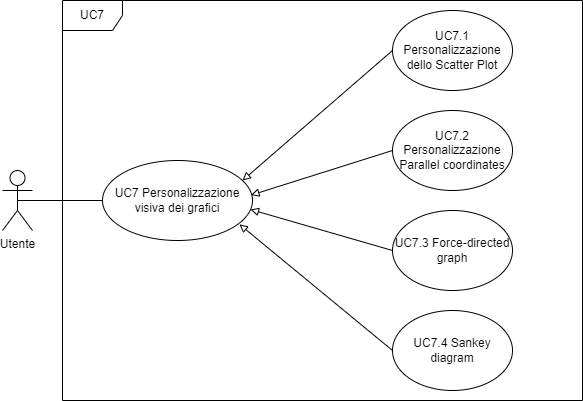
\includegraphics[scale=0.55]{../../assets/personalizzazioneVisivaGrafici.drawio.png}
	\caption{UC5 - Personalizzazione visiva dei grafici}
\end{figure}
\begin{itemize}
	\item \textbf{Attore primario:} Utente.
	\item \textbf{Precondizioni:} L'utente ha scelto uno dei grafici a disposizione nell'interfaccia [UC2].
	\item \textbf{Postcondizioni:} Il grafico viene ridisegnato secondo le scelte selezionate dall'utente.
	\item \textbf{Scenario principale:}
	\begin{enumerate}
    		\item L'utente seleziona il tipo di grafico e i colori che desidera e, per ogni elemento cambiato, i valori di default del grafico
    vengono cambiati. Nel caso si scelga di tornare alla vista di default, le modifiche eseguite torneranno ai valori standard.
    \end{enumerate}
    \item \textbf{Generalizzazioni}:
    \begin{itemize}
        \item L'utente seleziona una delle seguenti opzioni:
                \begin{enumerate}
                    \item \textit{Personalizza Scatter Plot} \hyperref[sec:UC5.1]{UC5.1}.
                    \item \textit{Personalizza Parallel Coordinates} \hyperref[sec:UC5.2]{UC5.2}.
                    \item \textit{Personalizza Force-directed Graph} \hyperref[sec:UC5.3]{UC5.3}.
                    \item \textit{Personalizza Sankey Diagram} \hyperref[sec:UC5.4]{UC5.4}.
                \end{enumerate}
    \end{itemize} 
\end{itemize}

% SCATTER PLOT
\newpage
\subsubsection{UC5.1 - Personalizzazione Scatter plot}
\label{sec:UC5.1}
\begin{figure}[h!]
	\centering
	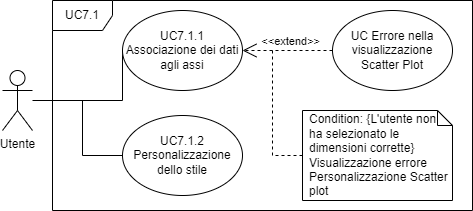
\includegraphics[scale=0.55]{../../assets/personalizzazioneScatterPlot.drawio.png}
	\caption{UC5 - Personalizzazione Scatter Plot}
\end{figure}
\begin{itemize}
    \item \textbf{Attore primario:} Utente.
	\item \textbf{Precondizioni:} L'utente ha scelto il grafico scatter plot. \hyperref[sec:UC2.1]{UC2.1}.
	\item \textbf{Postcondizioni:} 
	Il grafico viene ridisegnato secondo le scelte selezionate dall'utente.
	\item \textbf{Scenario principale:} L'utente decide:
	\begin{enumerate}
        \item Associazione delle dimensioni agli assi \hyperref[sec:UC5.1.1]{UC5.1.1}.
        \item Personalizzazione dello stile \hyperref[sec:UC5.1.2]{UC5.1.2}.
    \end{enumerate}
\end{itemize}
\paragraph{UC5.1.1 - Associazione delle dimensioni agli assi}
\label{sec:UC5.1.1}
    \begin{itemize}
        \item \textbf{Attore primario:} Utente.
        \item \textbf{Precondizioni:} L'utente ha selezionato lo scatter plot \hyperref[sec:UC2.1]{UC2.1}.
	    \item \textbf{Postcondizioni:} L'utente ha associato le dimensioni disponibili con gli assi del grafico.
	    \item \textbf{Scenario principale:} 
	    \begin{enumerate}
	    		\item L'utente sceglie quali dimensioni associare agli assi del grafico.
		\end{enumerate}
	    \item \textbf{Estensioni:} Nel caso l'utente non abbia associato correttamente le dimensioni agli assi del grafico:
              \begin{itemize}
                  \item Non viene visualizzato nessun grafico.
                  \item Viene visualizzato un errore di personalizzazione grafico \hyperref[sec:UC - Errore di personalizzazione]{UC?}.
              \end{itemize}
    \end{itemize}
\paragraph{UC5.1.2 - Personalizzazione dello stile}
\label{sec:UC5.1.2}
    \begin{itemize}
        \item \textbf{Attore primario:} Utente.
        \item \textbf{Precondizioni:} L'utente ha selezionato lo scatter plot \hyperref[sec:UC2.1]{UC2.1}.
	    \item \textbf{Postcondizioni:} L'utente ha selezionato tra le opzioni disponibili lo stile che preferisce.
	    \item \textbf{Scenario principale:} 
	    \begin{enumerate}
	    		\item L'utente visualizza le opzioni di colori per la personalizzazione di ogni specifica del grafico, nel caso l'utente non li modifichi rimangono quelli di default.
		\end{enumerate}
    \end{itemize}

% PARALLEL CORDINATES 
\subsubsection{UC5.2 - Personalizzazione Parallel coordinates}
\label{sec:UC5.2}
\begin{figure}[h!]
	\centering
	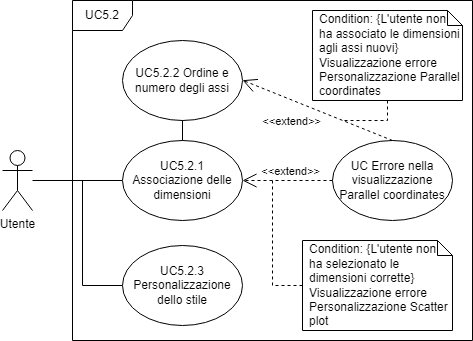
\includegraphics[scale=0.55]{../../assets/personalizzazioneParallelCoordinates.drawio.png}
	\caption{UC5 - Personalizzazione Parallel coordinates}
\end{figure}
\begin{itemize}
    \item \textbf{Attore primario:} Utente.
	\item \textbf{Precondizioni:} L'utente ha scelto il grafico Parallel coordinates. \hyperref[sec:UC2.1]{UC2.1}.
	\item \textbf{Postcondizioni:} Il grafico viene ridisegnato secondo le scelte selezionate dall'utente.
	\item \textbf{Scenario principale:} L'utente decide:
	\begin{enumerate}
        \item Associazione delle dimensioni \hyperref[sec:UC5.2.1]{UC5.2.1}.
        \item Ordine degli assi \hyperref[sec:UC5.2.2]{UC5.2.2}.
        \item Personalizzazione dello stile \hyperref[sec:UC5.2.3]{UC5.2.3}.
    \end{enumerate}
\end{itemize}

\paragraph{UC5.2.1 - Associazione delle dimensioni}
\label{sec:UC5.2.1}
    \begin{itemize}
        \item \textbf{Attore primario:} Utente.
        \item \textbf{Precondizioni:} L'utente ha selezionato Parallel coordinates. \hyperref[sec:UC2.2]{UC2.2}.
	    \item \textbf{Postcondizioni:} L'utente ha associato le dimensioni disponibili con gli assi del grafico.
	    \item \textbf{Scenario principale:}
	    \begin{enumerate}
	    		\item L'utente sceglie quali dimensioni associare agli assi del grafico.
		\end{enumerate}
	    \item \textbf{Estensioni:} Nel caso l'utente non abbia associato correttamente le dimensioni agli assi del grafico:
              \begin{itemize}
                  \item Non viene visualizzato nessun grafico.
                  \item Viene visualizzato un errore di visualizzazione personalizzazione grafico \hyperref[sec:UC - Errore di personalizzazione]{UC?}.
              \end{itemize}
    \end{itemize}
\paragraph{UC5.2.2 - Ordine e numero degli assi}
\label{sec:UC5.2.2}
    \begin{itemize}
        \item \textbf{Attore primario:} Utente.
        \item \textbf{Precondizioni:} L'utente ha selezionato Parallel coordinates. \hyperref[sec:UC2.2]{UC2.2}.
	    \item \textbf{Postcondizioni:} L'utente ha deciso un ordine degli assi e il loro numero.
	    \item \textbf{Scenario principale:} 
	    \begin{enumerate}
	    		\item L'utente sceglie ordine e numero degli assi.
		\end{enumerate}
	    \item \textbf{Estensioni:} Nel caso l'utente abbia creato nuovi assi ma non abbai associato nessuna dimensione ad essi:
              \begin{itemize}
                  \item Non viene visualizzato nessun grafico.
                  \item Viene visualizzato un errore di visualizzazione personalizzazione grafico.
              \end{itemize}
    \end{itemize}

\paragraph{UC5.2.3 - Personalizzazione dello stile}
\label{sec:UC5.2.3}
    \begin{itemize}
        \item \textbf{Attore primario:} Utente.
        \item \textbf{Precondizioni:} L'utente ha selezionato Parallel coordinates \hyperref[sec:UC2.2]{UC2.2}.
	    \item \textbf{Postcondizioni:} L'utente ha selezionato tra le opzioni disponibili lo stile che preferisce.
	    \item \textbf{Scenario principale:} 
	    \begin{enumerate}
	    		\item L'utente visualizza le opzioni di colori per la personalizzazione di ogni specifica del grafico, nel caso l'utente non li modifichi rimangono quelli di default.
		\end{enumerate}
    \end{itemize}


% FORCE-DIRECTED GRAPH 
\newpage
\subsubsection{UC5.3 - Personalizzazione Force-directed graph}
\label{sec:UC5.3}
\begin{figure}[h!]
	\centering
	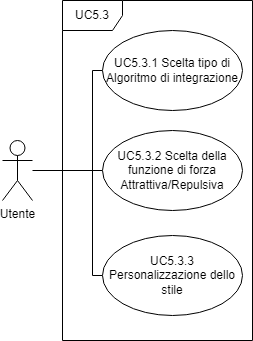
\includegraphics[scale=0.55]{../../assets/personalizzazioneForce-directedGraph.drawio.png}
	\caption{UC5 - Personalizzazione Force-directed graph}
\end{figure}
\begin{itemize}
    \item \textbf{Attore primario:} Utente.
	\item \textbf{Precondizioni:} L'utente ha scelto il grafico Force-directed graph. \hyperref[sec:UC2.3]{UC2.3}.
	\item \textbf{Postcondizioni:} Il grafico viene ridisegnato secondo le scelte selezionate dall'utente.
	\item \textbf{Scenario principale:}L'utente decide:
	\begin{enumerate}
        \item Associazione delle dimensioni \hyperref[sec:UC5.3.1]{UC5.3.1}.
        \item Ordine degli assi \hyperref[sec:UC5.3.2]{UC5.3.2}.
        \item Personalizzazione dello stile \hyperref[sec:UC5.3.3]{UC5.3.3}.
    \end{enumerate}
\end{itemize}
\paragraph{UC5.3.1 - Scelta tipo di algoritmo d'integrazione}
\label{sec:UC5.3.1}
    \begin{itemize}
        \item \textbf{Attore primario:} Utente.
        \item \textbf{Precondizioni:} L'utente ha selezionato Force-directed graph. \hyperref[sec:UC2.3]{UC2.3}.
	    \item \textbf{Postcondizioni:} L'utente ha associato l'algoritmo d'integrazione che desidera.
	    \item \textbf{Scenario principale:}
	    \begin{enumerate}
	    		\item L'utente sceglie l'algoritmo d'integrazione che desidera.
		\end{enumerate}
    \end{itemize}
\paragraph{UC5.3.2 - Scelta della funzione di forza}
\label{sec:UC5.3.2}
    \begin{itemize}
        \item \textbf{Attore primario:} Utente.
        \item \textbf{Precondizioni:} L'utente ha selezionato Force-directed graph. \hyperref[sec:UC2.3]{UC2.3}.
	    \item \textbf{Postcondizioni:} L'utente ha deciso i parametri per la rappresentazione.
	    \item \textbf{Scenario principale:} 
	    \begin{enumerate}
	    		\item L'utente sceglie i parametri per la rappresentazione dei rapporti tra i nodi.
		\end{enumerate}
	    \item \textbf{Estensioni:} Nel caso i parametri non rientrino nei limiti fissati:
              \begin{itemize}
                  \item Non viene visualizzato nessun grafico.
                  \item Viene visualizzato un errore di visualizzazione personalizzazione grafico \hyperref[sec:UC - Errore di personalizzazione]{UC?}.
              \end{itemize}
    \end{itemize}
\paragraph{UC5.3.3 - Personalizzazione dello stile}
\label{sec:UC5.3.3}
    \begin{itemize}
        \item \textbf{Attore primario:} Utente.
        \item \textbf{Precondizioni:} L'utente ha selezionato Force-directed graph \hyperref[sec:UC2.3]{UC2.3}.
	    \item \textbf{Postcondizioni:} L'utente ha selezionato tra le opzioni disponibili lo stile che preferisce.
	    \item \textbf{Scenario principale:} 
	    \begin{enumerate}
	    		\item L'utente visualizza le opzioni di colori per la personalizzazione di ogni specifica del grafico, nel caso l'utente non li modifichi rimangono quelli di default.
		\end{enumerate}
    \end{itemize}

% SANKEY DIAGRAM
\subsubsection{UC5.4 - Personalizzazione Sankey diagram}
\label{sec:UC5.4}
\begin{figure}[h!]
	\centering
	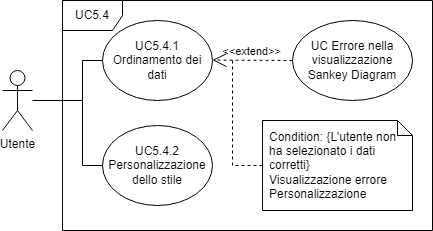
\includegraphics[scale=0.55]{../../assets/personalizzazioneSankey.drawio.png}
	\caption{UC5 - Personalizzazione Sankey diagram}
\end{figure}
\begin{itemize}
    \item \textbf{Attore primario:} Utente.
	\item \textbf{Precondizioni:} L'utente ha scelto il grafico Personalizzazione Sankey diagram. \hyperref[sec:UC2.4]{UC2.4}.
	\item \textbf{Postcondizioni:} Il grafico viene ridisegnato secondo le scelte selezionate dall'utente.
	\item \textbf{Scenario principale:}L'utente decide:
	\begin{enumerate}
        \item Ordinamento dei dati \hyperref[sec:UC5.4.1]{UC5.4.1}.
        \item Personalizzazione dello stile \hyperref[sec:UC5.4.2]{UC5.4.2}.
    \end{enumerate}
\end{itemize}
\paragraph{UC5.4.1 - Ordinamento dei dati}
\label{sec:UC5.4.1}
    \begin{itemize}
        \item \textbf{Attore primario:} Utente.
        \item \textbf{Precondizioni:} L'utente ha selezionato Sankey diagram. \hyperref[sec:UC2.3]{UC2.3}.
	    \item \textbf{Postcondizioni:} L'utente ha deciso le dimensioni da rappresentare.
	    \item \textbf{Scenario principale:}
	    \begin{enumerate}
	    		\item L'utente sceglie i parametri per la rappresentazione dei rapporti tra i nodi.
		\end{enumerate}
	    \item \textbf{Estensioni:} Nel caso i parametri non rientrino nelle relazioni fissate:
              \begin{itemize}
                  \item Non viene visualizzato nessun grafico.
                  \item Viene visualizzato un errore di visualizzazione personalizzazione grafico \hyperref[sec:UC - Errore di personalizzazione]{UC?}.
              \end{itemize}
    \end{itemize}
\paragraph{UC5.4.2 - Personalizzazione dello stile}
\label{sec:UC5.4.2}
\begin{itemize}
    \item \textbf{Attore primario:} Utente.
    \item \textbf{Precondizioni:} L'utente ha selezionato Sankey diagram \hyperref[sec:UC2.3]{UC2.3}.
	\item \textbf{Postcondizioni:} L'utente ha selezionato tra le opzioni disponibili lo stile che preferisce.
	\item \textbf{Scenario principale:}
	\begin{enumerate}
		\item L'utente visualizza le opzioni di colori per la personalizzazione di ogni specifica del grafico, nel caso l'utente non li modifichi rimangono quelli di default.
	\end{enumerate}
\end{itemize}

\newpage

% --------------------------------------------------------------------
% VISUALIZZAZIONE GRAFICO A TUTTO SCHERMO
% --------------------------------------------------------------------

\subsection{UC6 - Visualizzazione di un grafico a schermo intero}
\begin{figure}[h!]
	\centering
	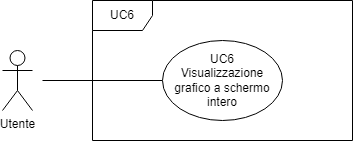
\includegraphics[scale=0.55]{../../assets/visualizzazione_fullscreen.png}
	\caption{UC6 - Visualizzazione di un grafico a schermo intero}
\end{figure}

\begin{itemize}
	\item \textbf{Attore primario:} Utente.
	\item \textbf{Precondizioni:} Il dataset è stato caricato correttamente. L'utente visualizza almeno un grafico sulla pagina. 
	\item \textbf{Postcondizioni:} 
	Viene mostrato il grafico scelto in \textit{fullscreen}.
	\item \textbf{Scenario principale:}
		\begin{enumerate}
			\item L'utente clicca sul pulsante di \textit{fullscreen} di un grafico.
			\item Il grafico viene visualizzato a schermo intero.
		\end{enumerate}
\end{itemize}
\newpage

% --------------------------------------------------------------------
% SEZIONE ZOOM INTERATTIVO
% --------------------------------------------------------------------

\subsection{UC7 - Zoom con selezione}
\label{sec:UC7}
\begin{figure}[h!]
    \centering
    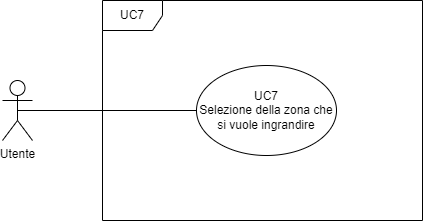
\includegraphics[scale=0.55]{../../assets/zoom_selezione.png}
    \caption{UC7 - Zoom con selezione sul grafico}
\end{figure}
\begin{itemize}
    \item \textbf{Attore primario}: Utente.
    \item \textbf{Precondizioni}: Il dataset è stato caricato correttamente. \par L'utente ha scelto la seguente tipologia di grafico:
    \begin{itemize}
    		\item \textit{Scatter Plot}.
    \end{itemize}
    \item \textbf{Postcondizioni}: Viene mostrato uno zoom della sezione selezionata dal mouse.
    \item \textbf{Scenario principale}:
          \begin{enumerate}
              \item L'utente seleziona con il mouse l'area all'interno del grafico che vuole ingrandire.
              \item L'area selezionata viene ingrandita.
          \end{enumerate}
\end{itemize}

\newpage

\subsection{UC7.1 - Zoom con scroll del mouse}
\label{sec:UC7.1}
\begin{figure}[h!]
    \centering
    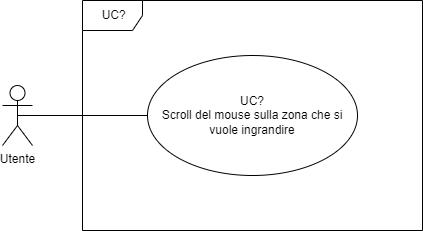
\includegraphics[scale=0.55]{../../assets/zoom_mouse.png}
    \caption{UC7.1 - Zoom con lo scroll del mouse}
\end{figure}
\begin{itemize}
    \item \textbf{Attore primario}: Utente.
    \item \textbf{Precondizioni}: Il dataset è stato caricato correttamente. \par L'utente ha scelto la seguente tipologia di grafico:
    \begin{itemize}
          \item \textit{Force-directed Graph}.
    \end{itemize}
    \item \textbf{Postcondizioni}: Viene mostrato uno zoom dove si trova il puntatore del mouse.
    \item \textbf{Scenario principale}:
          \begin{enumerate}
              \item L'utente posiziona il puntatore del mouse sulla zona di interesse.
              \item Per zoomare, l'utente esegue lo \textit{scroll} del mouse o utilizza le \textit{gesture} per lo zoom del \textit{trackpad}.
              \item L'area selezionata viene ingrandita.
          \end{enumerate}
\end{itemize}

\newpage

% --------------------------------------------------------------------
% SEZIONE MOUSE HOVER
% --------------------------------------------------------------------
\subsection{UC8 - Mouse Hover}
\label{sec:UC8}
\begin{figure}[h!]
    \centering
    % Controlla che UC abbia il numero corretto
    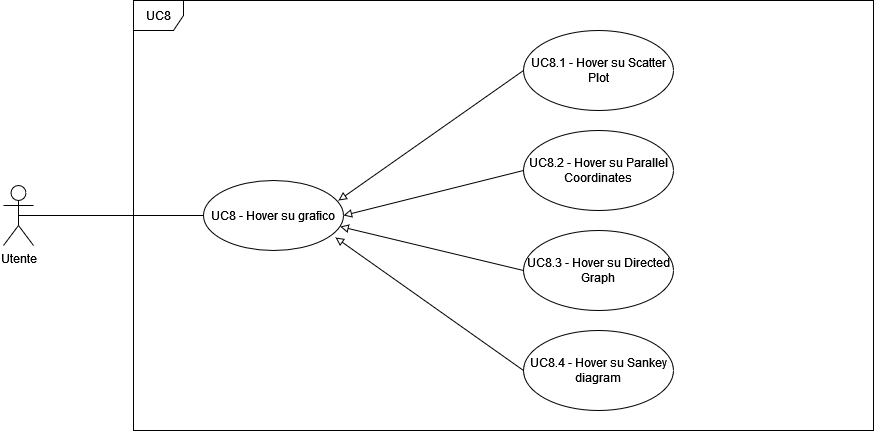
\includegraphics[scale=0.55]{../../assets/UC8-MouseHover.png}
    \caption{UC8 - Mouse Hover}
\end{figure}
\begin{itemize}
    \item \textbf{Attore primario:} Utente.
    \item \textbf{Precondizioni:} Il dataset è stato caricato correttamente. L'utente ha scelto quale tipologia di grafico visualizzare e ha selezionato una vista.
    \item \textbf{Postcondizioni:} Vengono mostrate all'utente informazioni utili relative all'elemento su cui il mouse sta eseguendo l'hover.
    \item \textbf{Scenario principale}: 
    \begin{enumerate}
		\item L'utente passa con il mouse sopra ad un elemento di interesse. 
		\item Visualizza delle informazioni utili.
		\item L'elemento viene evidenziato. 
	\end{enumerate}
	Tutto ciò dipende chiaramente su quale grafico l'utente sta eseguendo la funzione di hover.
    \item \textbf{Generalizzazioni:} \begin{enumerate}
                                        \item Hover su \textit{Scatter Plot} [\hyperref[sec:UC8.1]{UC8.1}]
                                        \item Hover su \textit{Parallel coordinates} [\hyperref[sec:UC8.2]{UC8.2}]
                                        \item Hover su \textit{Force-directed graph} [\hyperref[sec:UC8.3]{UC8.3}]
                                        \item Hover su \textit{Sankey diagram} [\hyperref[sec:UC8.4]{UC8.4}]
                                    \end{enumerate}
\end{itemize}

\subsubsection{UC8.1 - Hover su Scatter Plot}
\label{sec:UC8.1}
\begin{itemize}
    \item \textbf{Attore primario:} Utente.
    \item \textbf{Precondizioni:} Il dataset è stato caricato correttamente. L'utente ha scelto di visualizzare il grafico \textit{Scatter Plot} e ha selezionato una vista.
    \item \textbf{Postcondizioni:} L'utente passando sopra con il mouse ad un punto sul grafico ottiene più informazioni relative a quel punto e lo evidenzia.
    \item \textbf{Scenario principale}: 
    \begin{enumerate}
		\item L'utente passa con il mouse sopra ad un punto sul grafico.
		\item Visualizza un'etichetta che contiene informazioni più complete relative a quel punto, come ad esempio: valore delle coordinate delle x, valore delle coordinate delle y etc. 
		\item Viene evidenziato il punto rispetto a tutti gli altri.
	\end{enumerate}
\end{itemize}

\subsubsection{UC8.2 - Hover su Parallel Coordinates}
\label{sec:UC8.2}
\begin{itemize}
    \item \textbf{Attore primario:} Utente.
    \item \textbf{Precondizioni:} Il dataset è stato caricato correttamente. L'utente ha scelto di visualizzare il grafico \textit{Parallel Coordinates} e ha selezionato una vista.
    \item \textbf{Postcondizioni:} L'utente passando sopra con il mouse a una linea o a un gruppo di linee ottiene maggiori informazioni a riguardo.
    \item \textbf{Scenario principale}:
    \begin{enumerate}
		\item L'utente passa con il mouse sopra ad una linea o ad un gruppo di linee sul grafico.
		\item Visualizza un'etichetta che contiene informazioni più complete relative a quella linea o a quel gruppo di linee.
		\item Vengono evidenziati la linea o il gruppo intero.
	\end{enumerate}
\end{itemize}

\subsubsection{UC8.3 - Hover su Force-directed Graph}
\label{sec:UC8.3}
\begin{itemize}
    \item \textbf{Attore primario:} Utente.
    \item \textbf{Precondizioni:} Il dataset è stato caricato correttamente. L'utente ha scelto di visualizzare il grafico \textit{Force-directed Graph} e ha selezionato una vista.
    \item \textbf{Postcondizioni:} L'utente passando sopra con il mouse a un nodo del grafo lo evidenzia ed ottiene maggiori informazioni a riguardo.
    \item \textbf{Scenario principale}:
    \begin{enumerate}
		\item L'utente passa con il mouse sopra ad un nodo del grafo.
		\item Visualizza un \textit{tooltip} che mostra maggiori informazioni a riguardo.
		\item Viene evidenziato il nodo.
	\end{enumerate}
\end{itemize}

\subsubsection{UC8.4 - Hover su Sankey Diagram}
\label{sec:UC8.4}
\begin{itemize}
    \item \textbf{Attore primario:} Utente.
    \item \textbf{Precondizioni:} Il dataset è stato caricato correttamente. L'utente ha scelto di visualizzare il grafico \textit{Sankey Diagram} e ha selezionato una vista.
    \item \textbf{Postcondizioni:} L'utente passando sopra con il mouse ad elemento nel grafico lo evidenzia.
    \item \textbf{Scenario principale}: 
    \begin{enumerate}
		\item L'utente passa con il mouse sopra ad un nodo del grafo.
		\item Vengono evidenziati il nodo ed i collegamenti da lui entranti e uscenti.
		\item L'utente passa con il mouse sopra ad un collegamento.
		\item Viene evidenziato il collegamento.
	\end{enumerate}
\end{itemize}

\newpage

% --------------------------------------------------------------------
% SEZIONE UC9 - CREAZIONE NUOVA VISTA DA FARE
% --------------------------------------------------------------------


% --------------------------------------------------------------------
% SEZIONE SALVATAGGIO VISTA SU FILE
% --------------------------------------------------------------------

\subsection{UC10 - Salvataggio vista}
\label{sec:UC10}
\begin{figure}[h!]
    \centering
    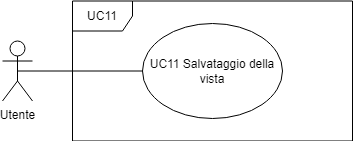
\includegraphics[scale=0.55]{../../assets/salvataggio_vista.png}
    \caption{UC10 - Salvataggio della vista su file}
\end{figure}
\begin{itemize}
    \item \textbf{Attore primario}: Utente.
    \item \textbf{Precondizioni}: Il dataset è stato caricato correttamente. L'utente ha scelto una tipologia di grafico e ha creato una propria vista personalizzata.
    \item \textbf{Postcondizioni}: La vista viene salvata all'interno di un file \textit{.json}.
    \item \textbf{Scenario principale}:
          \begin{enumerate}
              \item L'utente seleziona il pulsante di salvataggio della vista.
              \item Il file viene scaricato in locale in formato \textit{.json}.
          \end{enumerate}
\end{itemize}

\newpage

\subsection{UC11 - Caricamento vista}
\label{sec:UC11}
\begin{figure}[h!]
    \centering
    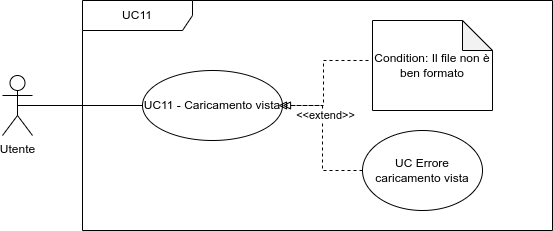
\includegraphics[scale=0.55]{../../assets/caricamento_vista.png}
    \caption{UC10 - Salvataggio della vista su file}
\end{figure}
\begin{itemize}
    \item \textbf{Attore primario}: Utente.
    \item \textbf{Precondizioni}: Il dataset è stato caricato correttamente.
    \item \textbf{Postcondizioni}: È selezionabile la nuova vista nel menù viste descritto da UC3.
    \item \textbf{Scenario principale}:
          \begin{enumerate}
              \item L'utente preme il pulsante "carica vista".
              \item L'utente seleziona il file \textit{.json} contenente la vista.
              \item L'applicativo rende disponibile la vista appena caricata.
          \end{enumerate}
    \item \textbf{Estensioni:}
    \begin{itemize}
        \item Nel caso il json contenente la vista non sia ben formato: \begin{enumerate}
            \item La vista non viene caricata.
            \item Viene visualizzato un messaggio d'errore.
        \end{enumerate}
    \end{itemize}
\end{itemize}

\newpage
% --------------------------------------------------------------------
% SEZIONE ERRORI
% --------------------------------------------------------------------

\section{Errori}
\subsection{UC - Errore formato file}
\label{sec:UC - Errore formato file}
\begin{itemize}
    \item \textbf{Attore primario:} Utente
    \item \textbf{Precondizioni:} L'utente carica un file in un formato non supportato.
    \item \textbf{Postcondizioni:} L'utente visualizza un messaggio di errore e il file non viene caricato.
    \item \textbf{Scenario principale:}
          \begin{enumerate}
              \item L'utente visualizza un messaggio di errore esplicativo
              \item L'utente clicca "OK" per proseguire.
          \end{enumerate}
\end{itemize}

\subsection{UC - Errore struttura dataset}
\label{sec:UC - Errore struttura dataset}
\begin{itemize}
    \item \textbf{Attore primario:} Utente
    \item \textbf{Precondizioni:} L'utente carica un file nel formato supportato ma che non è correttamente strutturato  
                                  (e.g. due o più colonne sono invertite oppure una o più colonne sono mancanti). 
    \item \textbf{Postcondizioni:} L'utente visualizza un messaggio di errore e il file non viene caricato.
    \item \textbf{Scenario principale:}
          \begin{enumerate}
              \item L'utente visualizza un messaggio di errore esplicativo.
              \item L'utente clicca "OK" per proseguire.
          \end{enumerate} 
\end{itemize}

\subsection{UC - Errore validità riga nel dataset}
\label{sec:UC - Errore validità riga}
\begin{itemize}
    \item \textbf{Attore primario:} Utente
    \item \textbf{Precondizioni:} L'utente carica un file nel formato supportato e ben strutturato ma una o più righe presentano un dato non valido (e.g. nella colonna relativa ai \textit{timestamp} il valore è negativo).  
    \item \textbf{Postcondizioni:} L'utente visualizza un messaggio di errore che chiede se ignorare la riga non valida, oppure continuare.
    \item \textbf{Scenario principale:}
    \begin{itemize}
        \item   L'utente sceglie di ignorare la riga:
                \begin{enumerate}
                    \item L'utente visualizza un messaggio di errore esplicativo.
                    \item L'utente clicca "IGNORA" per ignorare la riga non valida.
                    \item Il file viene caricato escludendo la riga precedentemente ignorata.
                \end{enumerate} 
        \item   L'utente sceglie di proseguire:
                \begin{enumerate}
                    \item L'utente visualizza un messaggio di errore esplicativo.
                    \item L'utente clicca "OK" per proseguire.
                    \item Il file non viene caricato.
                \end{enumerate} 
    \end{itemize}
\end{itemize}

\subsection{UC - Errore di visualizzazione personalizzazione grafico}
\label{sec:UC - Errore di personalizzazione}
\begin{itemize}
    \item \textbf{Attore primario:} Utente
    \item \textbf{Precondizioni:}
    		\begin{itemize}
    			\item L'utente associa non correttamente una o più dimensioni ad uno o più assi nel grafico.
    			\item L'utente inserisce dei parametri relativi alla funzione di forza non corretti.
    			\item L'utente sceglie dei parametri relativi all'ordinamento dei dati non corretti.
    		\end{itemize}
    \item \textbf{Postcondizioni:} L'utente visualizza un messaggio d'errore esplicativo relativo alla condizione che ha causato l'errore, e le modifiche da lui apportate non vengono eseguite.
    \item \textbf{Scenario principale:}
    \begin{enumerate}
        \item L'utente visualizza un messaggio di errore esplicativo.
        \item L'utente clicca "OK" per proseguire.
    \end{enumerate}
\end{itemize}

\subsection{UC - Errore caricamento vista}
\label{sec:UC - Errore caricamento vista}
\begin{itemize}
    \item \textbf{Attore primario:} Utente
    \item \textbf{Precondizioni:}
    		\begin{itemize}
    			\item L'utente carica un file vista non ben formato.
    		\end{itemize}
    \item \textbf{Postcondizioni:} L'utente visualizza un messaggio d'errore esplicativo relativo alla condizione che ha causato l'errore, non viene caricata la vista.
    \item \textbf{Scenario principale:}
    \begin{enumerate}
        \item L'utente visualizza un messaggio di errore esplicativo.
        \item L'utente clicca "OK" per proseguire.
    \end{enumerate}
\end{itemize}
